
\section{Introduction and Problem Domain}
\label{sec:intro}
The core research question of this study investigates whether continuously computed and maintained semantic context can fundamentally resolve the geometric and computational bottlenecks inherent to traditional Retrieval-Augmented Generation (RAG).

\subsection{The Architectural Limits of Standard RAG}
Traditional RAG systems treat context assembly as a strictly query-time operation. When a user issues a query, the system embeds the text, performs an Approximate Nearest Neighbor (ANN) search over an unstructured Vector Database, retrieves $K$ discrete text chunks, and concatenates them into an LLM's prompt window. 

While effective for localized, single-document retrieval, this architecture catastrophically degrades in complex enterprise environments. First, unstructured vector similarity search inherently suffers from $O(N)$ scalability limits. As the enterprise corpus $N$ scales, the geometric distance between semantic concepts begins to collapse, leading to "embedding dilution".

\begin{figure*}[htbp]
\centering
\resizebox{\linewidth}{!}{
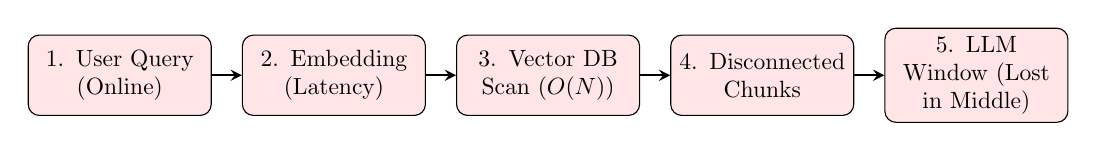
\begin{tikzpicture}[
    node distance=3.2cm, auto, scale=0.85, transform shape,
    box/.style={rectangle, draw, fill=red!10, text width=2.5cm, text centered, rounded corners, minimum height=1.2cm},
    arrow/.style={thick,->,>=stealth}
]
\node (query) [box] {1. User Query (Online)};
\node (embed) [box, right of=query] {2. Embedding (Latency)};
\node (vdb) [box, right of=embed] {3. Vector DB Scan ($O(N)$)};
\node (chunks) [box, right of=vdb] {4. Disconnected Chunks};
\node (llm) [box, right of=chunks] {5. LLM Window (Lost in Middle)};

\draw [arrow] (query) -- (embed);
\draw [arrow] (embed) -- (vdb);
\draw [arrow] (vdb) -- (chunks);
\draw [arrow] (chunks) -- (llm);
\end{tikzpicture}
}
\caption{Standard RAG Architecture. The linear $O(N)$ retrieval bottleneck occurs entirely at query time.}
\label{fig:rag_issues}
\end{figure*}

Second, standard RAG fails at cross-system multi-hop reasoning. If an answer requires linking a Slack message to a Jira ticket, traditional RAG must either rely on the LLM's internal reasoning to bridge the chunks, or employ iterative agentic loops which compound latency.
